\documentclass[a4paper,12pt]{article}

% Pakete
\usepackage[utf8]{inputenc}
\usepackage[english]{babel} % Deutsche Sprache
\usepackage{graphicx} % Für Bilder
\usepackage{amsmath} % Für mathematische Formeln
\usepackage{booktabs} % Für Tabellen
\usepackage[hidelinks]{hyperref} % Für Hyperlinks
\usepackage{listings} % Für Code-Blöcke
\usepackage{minted} % Auch für Code-Blöcke
\usepackage{caption}
\usepackage{menukeys}
\usepackage{float}
\usepackage{enumitem}
\usepackage{tocloft}
\usepackage{pgfplots}
\usepackage{pgfplotstable}
\usepgfplotslibrary{groupplots}
\usepackage{siunitx}
\usepackage{multicol}
\usepackage{xcolor}
\usepackage{tikz}
\usepackage{textcomp}
\newcommand{\mytexttilde}{\raisebox{0.5ex}{\texttildelow}}

\usepackage{fancyhdr}
\pagestyle{fancy}

\fancyhf{} % löscht alle aktuellen Kopf- und Fußzeilen

% Kopfzeile: linke Seite = aktuelle Section
\fancyhead[L]{\nouppercase{\leftmark}}

% Fußzeile: linke Seite = Name, rechte Seite = FH Salzburg, zentriert = Seitenzahl
\fancyfoot[L]{Marc Toiflhart, Sebastian Maier}
\fancyfoot[C]{\thepage}
\fancyfoot[R]{Högskolan i Halmstad}

\usepackage{placeins}

\usepackage[
backend=biber,
style=ieee,
sorting=ynt
]{biblatex}

\renewcommand{\listingscaption}{Sourcecode}

\addbibresource{literatur.bib}

\begin{document}

\begin{titlepage}
    \centering
    
\includegraphics[width=5cm]{Resources/hogskolan-halmstad-logo.png} \\[0.5cm] % Logo
    Högskolan i Halmstad \\[0.2cm]
    Biometric Recognition \\[1.5cm]
    
    \hrule
    \vspace{0.4cm} % statt \\[0.4cm]
    {\LARGE \textbf{Laboratory Report}}
    \vspace{0.4cm}
    \hrule
    \vspace{1.5cm} % statt \\[1.5cm]

    {\Large \textbf{Biometric Recognition Laboratory}} \\[0.2cm]
    {\Large Hand Geometry} \\[1cm]
    
    \textbf{Author:} Marc Toiflhart, Sebastian Maier \\[0.2cm]
    \textbf{Date:} \today \\[0.2cm]
    \textbf{Supervisor:} Kevin Hernández Diaz

    \vfill
\end{titlepage}
\newpage

\begin{center}
    \textbf{Summary}
\end{center}
In diesem Labor wurden Videosequenzen mit dem H.264-Codec unter variierenden Bitraten, Quantisierungsparametern und Presets kodiert und hinsichtlich Qualität und Kodierzeit analysiert. Ergänzend wurde ein C-Programm zur Einlesung und Verifikation von IYUV-Daten sowie zur Motion Estimation mit verschiedenen Metriken entwickelt.

\vspace{0.4cm} % statt \\[0.4cm]
\centering
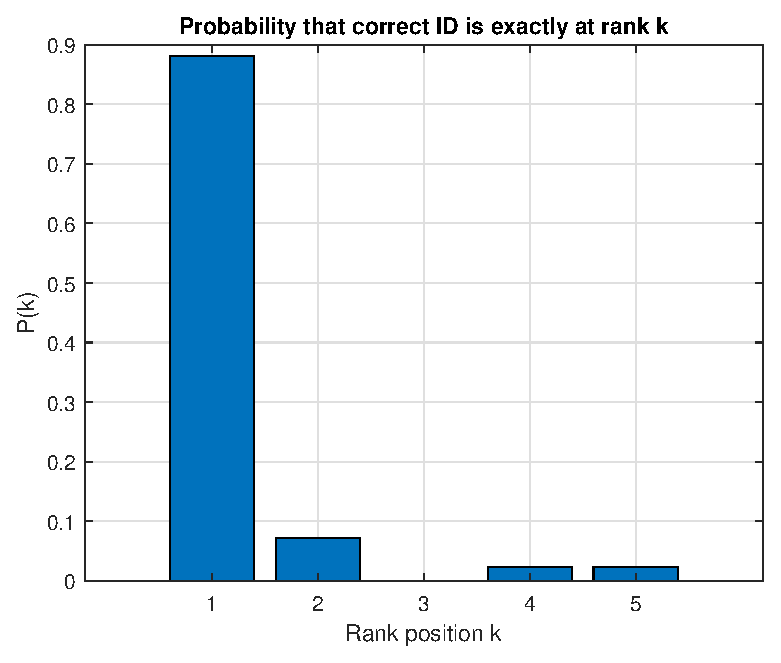
\includegraphics[width=5cm]{Resources/rank_plot.eps} \\[0.5cm]

% Inhaltsverzeichnis
\tableofcontents
\newpage

% Abbildungsverzeichnis
\listoffigures
\newpage

% Tabellenverzeichnis
\listoftables
\newpage

\captionsetup{type=listing}
\begin{minted}[linenos,tabsize=2,breaklines]{bash}
#!/bin/bash
bitrates=( 100 200 500 )

if [ $# -ne 2 ]; then
	echo "Usage: $0 <input_file> <output_dir>"
	exit 1
fi

input_file=$1
output_dir=$2

mkdir -p "$output_dir"

# Basisname ohne Dateiendung extrahieren
base_name=$(basename "$input_file")
base_name="${base_name%.*}"

for bitrate in ${bitrates[@]}
do
	output_file="${output_dir}/${base_name}_${bitrate}.264"
	x264 -o "$output_file" --input-res 352x288 --bitrate $bitrate "$input_file"
done
\end{minted}
\captionof{listing}{Bash-Script zum Erzeugen der Videodateien unter x264 mit unterschiedlichen Bitraten}
\label{lst:bashscript_x264_bitrates}
\vspace{10pt}

\newpage
\printbibliography

\end{document}